\subsection{UC-15}
\label{subsec:UC-15}


\begin{figure}[H]
    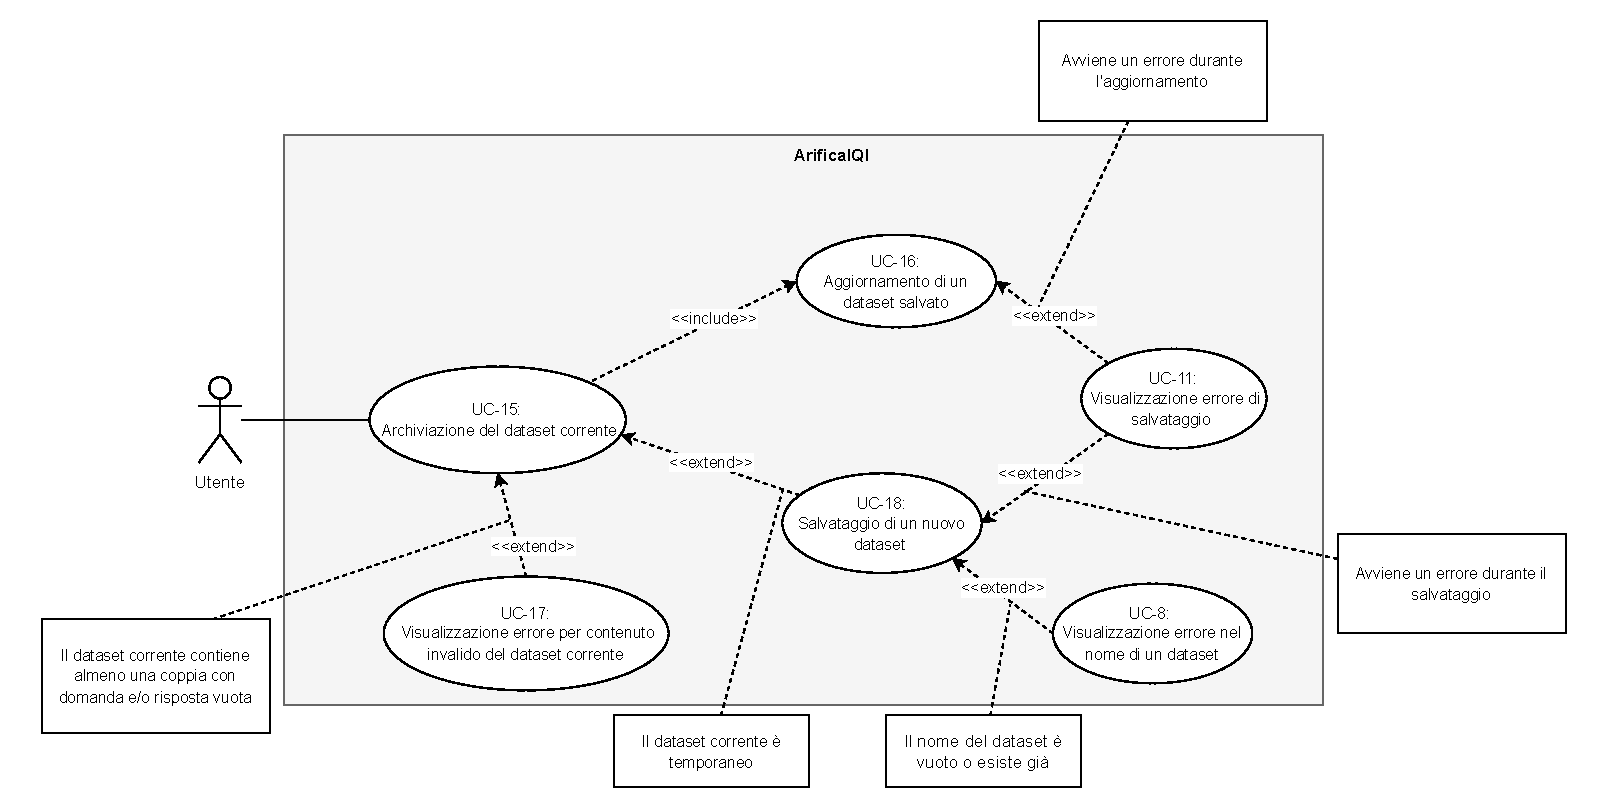
\includegraphics[scale=0.75]{Sezioni/UseCase/Immagini/UC-15.pdf}
    \caption{Diagramma UC-15.}
\end{figure}

\begin{usecase}{UC-15}{Archiviazione del dataset caricato}
    
    \req{\hyperref[item:RU-5]{RU-5}} 

    \pre{
        \item Il sistema è attivo e funzionante
        \item Il dataset caricato non è vuoto
    }

    \post{
        \item Il dataset caricato viene archiviato nel sistema
    }
    
    \actor{Utente}

    \subactors{}

    \trigger{L'utente deve archiviare il dataset caricato per renderlo persistente}
    
    \inc{\hyperref[subsec:UC-16]{UC-16}}

    \base{}

    \scenario{
        \item L'utente richiede l'archiviazione del dataset caricato.
        \item \texttt{<<include:UC-16>>}
    }

    \subscenario{
        \item[1.1] \textbf{Il dataset caricato contiene almeno una coppia con domanda e/o risposta vuota}
        \begin{itemize}
            \item[a.] \hyperref[subsec:UC-17]{UC-17}
        \end{itemize}
        \item[1.2] \textbf{Il dataset caricato è temporaneo perchè è stato appena creato}
        \begin{itemize}
            \item[a.] 
        \end{itemize}
    }
\end{usecase}
